\chapter{
روش تی اس ان ای
}
در فصل قبلی به توضیح روش اس ان ای پرداختیم، با اینکه روش اس ان ای مصور سازی خوبی ارائه می‌دهد اما عملکرد این روش توسط تابع هزینه‌ای که به سختی بهینه می‌شود و مشکلی به نام مشکل شلوغی، کاهش یافته است.
در این بخش ما به بررسی روش تی اس ان ای می‌پردازیم که سعی دارد این مشکلات را حل کند.
\\
تابع هزینه این روش دو تفاوت اساسی با تابع هزینه‌ی روش اس ان ای دارد، اولین تفاوت این است که در این روش از نسخه‌ی متقاران تابع اس ان ای برا گرادیانی ساده‌تر استفاده می‌کنیم و دومین تفاوت این است که برای محاسبه‌ی شباهت بین داده‌های کم بعد، به جای توزیع گوسی از
 {توزیع t استیودنت}\LTRfootnote{Student-t distribution}
استفاده می‌شود
\\
روش تی اس ان ای از توزیع‌
 {دم سنگین}\LTRfootnote{heavy-tailed distribution}
برای ابعاد کوچک استفاده می‌کند که دو مشکل بهینگی و مشکل شلوغی در اس ان ای را حل نماید.
\\
در این فصل ابتدا به نسخه‌ی متقارن اس ان ای می‌پردازیم، سپس مشکل شلوغی را مطرح کرده و پس از آن نحوه استفاده از توزیع‌های دم سنگین برای حل این مشکل را بیان می‌کنیم، در نهایت روش‌های مطرح شده برای حل مشکل بهینگی اس ان ای بیان می‌شود.
\section{اس ان ای متقارن}
برای یک جایگزین برای مینیمم کردن تابع واگرایی کولبک-لیبلر بین توابع احتمالی شرطی
$p{j|i}$
و
$q_{j|i}$
می‌توان سعی کرد که یک تابع واگرایی کولبک-لیبلر بین توزیع $P$ در ابعاد بالا و توزیع $Q$ در ابعاد پایین استفاده نمود.
فرمول تابع هزینه جدید به این شکل می‌شود:
\begin{figure}[!h]
	\centering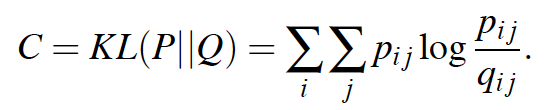
\includegraphics[scale=.3]{eq8}
	\caption{تابع هزینه متقاران}\label{fig.eq8}
\end{figure}
\\
که باز در این تابع نیز مقادیر $p_{ii}$ و $q_{ii}$ برابر با صفر هستند.
این نوع اس ان ای، اس ان ای متقارن شمرده می‌شود زیرا برای تمام $i$ و $j$ ها داریم که
$p_{ij} = p_{ji}$
و 
$q_{ij} = q_{ji}$
.
\\
در اس ان ای متقارن، شباهت بین دو نقطه نگاشت شده در ابعاد پایین با فرمول زیر محاسبه می‌شود:
 \begin{figure}[!h]
 	\centering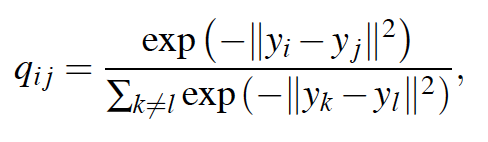
\includegraphics[scale=.3]{eq9}
 	\caption{تابع شباهت در ابعاد پایین}\label{fig.eq9}
 \end{figure}
\\
و همچنین تابع شباهت بین دو نقطه در ابعاد بالا نیز به فرمول زیر است:
\begin{figure}[!h]
	\centering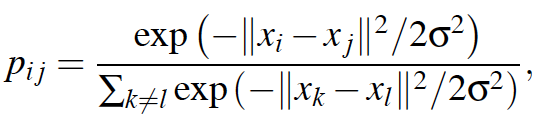
\includegraphics[scale=.3]{eq10}
	\caption{تابع شباهت در ابعاد بالا}\label{fig.eq10}
\end{figure}
\\
اما این فرمول در زمانی که یک داده در ابعاد بالا،
{داده‌ی پرت}\LTRfootnote{outlier}
باشد مشکل زا می‌شود زیرا مقدار $p_{ij}$ برای تمام $j$ های به غیر از این داده بسیار کم می‌شود و نگاشت آن به هر جایی از صفحه آنچنان تاثیری در تابع هزینه نخواهد داشت و در نتیجه مکان این نقطه نگاشت شده، به خوبی توسط بقیه نقاط مشخص نمی‌شود.
\\
برای دور زدن این مشکل، تابع شباهت در ابعاد بالا را به صورت میانگین دو تابع احتمال شرطی تعریف می‌کنیم، یعنی مقدار $p_{ij}$ را به صورت
$\frac{p_{j|i} + p_{i|j}}{2n}$
تعریف می‌کنیم. این تعریف تضمین می‌دهد که
$\sum_j {p_{ij}} > \frac{1}{2n}$
برای تمام
$x_i$
ها و در نتیجه هر نقطه، تاثیر بالایی در تابع هزینه $C$ خواهد داشت.
\\
تابع شباهت برای ابعاد پایین را تغییر نمی‌دهیم زیرا مشکل قبلی پیش نخواهد آمد.
\\
برتری اصلی اس ان ای متقارن نسبت به اس ان ای معمولی این است که تابع گرادیان آن بسیار ساده‌تر است که این موضوع باعث می‌شود که محاسبه‌ی آن بسیار سریع‌تر باشد. تابع گرادیان برای اس ان ای متقارن به شکل زیر است:
\begin{figure}[!h]
	\centering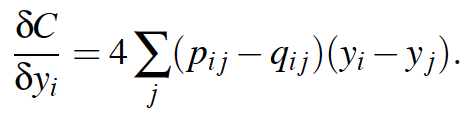
\includegraphics[scale=.3]{eq11}
	\caption{تابع گرادیان برای اس ان ای متقارن}\label{fig.eq11}
\end{figure}
\\
نتایج آزمایش‌ها نشان می‌دهد که اس ان ای متقارن قالبا همان نگاشت اس ان ای را خروجی می‌دهد و گاها عملکرد بهتری نیز ارائه می‌دهد.

\section{مشکل شلوغی}
مجموعه‌ای از نقاط دو بعدی را در نظر بگیرید، که بر روی یک منحی دو بعدی نامتقارن و دارای پستی و بلندی قرار دارند که در به صورت تقریبی می‌توان با یک خط در اندازه‌های کوچک تقریب زده شوند، و تمام این نقاط در فضایی با ابعاد بالا تعبیه شده‌اند.
این امکان وجود دارد که فاصله‌ی دو به دوی نقاط را در یک نگاشت دو بعدی مدل کرد.
\\
حال فرض کنید که پستی بلندی‌های واقعی منحنی که در نگاه جزئی دیده نمی‌شدند دارای ده بعد دیگر جز این دو بعد باشند که دیگر نمی‌توان آن‌ها را به خوبی در دو بعد مدل کرد. دلایل متنوعی برای این موضوع وجود دارد که برای مثال می‌توان گفت که در ۱۰ بعد، می‌توان ۱۱ نقطه را جوری در صفحه چید که فاصله‌ی بین آن‌ها را به هیچ صورتی نمی‌توان به خوبی در دو بعد نشان داد.
\\
یک مسئله مربوط به این موضوع، مسئله‌ی نگاشت یک ابر کره‌ی $m$ بعدی به دو بعد است که توزیع نقاط در آن به این صورت است که یک مرکز در نظر گرفته شده و احتمال وجود یه نقطه در مکانی که فاصله‌ی $r$ از مرکز دارد متناسب با $r^m$ می‌باشد، که برای حل این مسئله نیز به مشکل شلوغی می‌خوریم.
\\
مسئله شلوغی رو می‌توانیم به این صورت تعریف کنیم: فضای دو بعدی در دسترس برای نمایش فاصله‌ی نقاط نسبتا دور از هم به اندازه‌ی کافی بزرگتر از فضای دو بعدی در دسترس برای نمایش فاصله‌ی نقاط نزدیک به هم نیست، به همین دلیل ما اگر بخواهیم فاصله‌ی نقاط نزدیک به هم را به خوبی نگاشت دهیم، نقاط نسبتا دور از هم در نگاشت، بسیار دور از هم نگاشت داده می‌شوند.
\\
در اس ان ای، فنری که بین این داده‌ی $i$ و هر یک از این داده‌های بسیار دور نگاشت داده شده، قرار داده شده است، بسیار  سختی پایینی دارد و به همین دلیل نیروی جذبی ضعیفی از خود نشان می‌دهد.
\\
اگرچه این فنرها نیروهای بسیار ضعیفی از خود نشان می‌دهند اما تعداد زیادی از این نیرو‌ها داده‌ها را به سمت مرکز حرکت می‌دهد که باعث می‌شود فاصله‌ی طبیعی بین خوشه‌ها از بین برود.
\\
دقت کنید که این مشکل فقط مربوط به اس ان ای نمی‌باشد و در روش‌های دیگر نیز پیش می‌آید.
\\
یک تلاش برای حل مشکل شلوغی، اضافه کردن یک دافعه خفیف به هر فنر می‌باشد.
\\
این دافعه خفیف به این شکل ساخته می‌شود که یک مدل پس‌زمینه یکنواخت با نسبت اختلاط $\rho$ معرفی می‌شود. که در آن نقاط نگاشت داده شده‌ی بسیار دور از هم مقدار $q_{ij}$ کمتر از 
$\frac{2p}{n(n-1)}$
نمی‌توانند داشته باشند که در نتیجه‌ی آن نقاطی که در ابعاد بالا بسیار دور هستند مقدار $q_{ij}$ آن‌ها همواره بیشتر از مقدار $p_{ij}$ آن‌ها می‌شود که این موضوع باعث یک دافعه خفیف می‌شود.
\\
به این روش
{یونی اس ان ای}\LTRfootnote{UNI-SNE}
می‌گویند که گرچه بسیار بهتر از روش اس ان ای عمل می‌کند اما تابع هزینه‌ی آن بسیار پیچیده است.
\section{دم نامناسب می‌تواند ابعاد ازبین رفته را جبران کند}
از آنجایی که روش اس‌ان‌ای متقارن تلاش می‌کند تا توزیع توأم در ابعاد بالا و پایین را برابر یک‌دیگر قرار دهد، راه حل مناسبی برای حل مشکل گزارش شده در زیر بخش قبل وجود دارد که به شرح زیر است.
در ابعاد بالا برای تبدیل فاصله به احتمال از توزیع گوسی استفاده‌شده‌است اما در ابعاد‌پایین می‌توان از توزیع احتمالی استفاده کرد که فاصله خطی بیش‌تری را نسبت به توزیع گوسی ایجاد کند. با این‌روش فاصه‌های که متوسط هستند نیز در ابعاد کوچک به فاصله‌های بزرگ‌تر مپ می‌شوند و به طبع باعث می‌شود که آن‌های که در یک خوشه نیستند شباهت احتمالی کمتری داشته‌باشند و نمایش بهتری داشته باشیم.

\section{روش‌های بهینه‌سازی برای تی-اس‌ان‌ای}
در ابتدا روش تی-‌اس‌ان‌ای با استفاده از الگوریتم گرادیان‌دسنت روی تابع‌هزینه بهینه‌سازی شد. شبه کد نحوه‌ی بهینه سازی آن در\cref{algfig1} آورده شده است.
\\
\begin{figure}
	\centering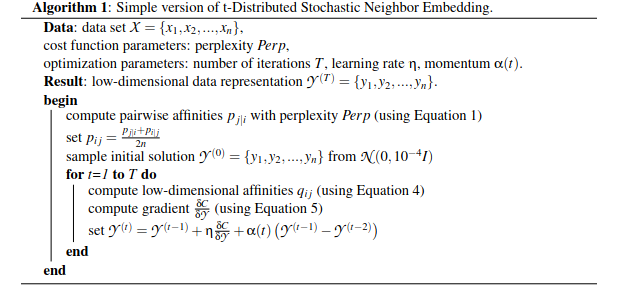
\includegraphics[scale=.6]{algfig1.png}
	\caption{شبه کد بهینه سازی }\label{algfig1}
\end{figure}

این الگوریتم ساده این قابلیت‌را دارد تا با استفاده از  نرخ‌یادگیری‌انطباقی که در سال ۱۹۸۸ توسط جکابس \LTRfootnote{Jcobs }معرفی شد، که در آن نرخ یادگیری را درجهتی که گرادیان ثابت بماند، نرخ یادگیری را زیاد‌میکرد ،سریع‌تر شود.
\\
هرچند این الگوریتم تصاویری ایجاد می‌کند که بسیار بهتر از دیگر الگوریتم‌های غیر‌پارامتریک هستند،  می‌توان از طریق دو ایده‌ای که در این بخش معرفی‌می‌کنیم تصاویر بسیار بهتری ایجاد کرد.
اولین ایده که آن‌را فشرده‌سازی‌اولیه \LTRfootnote{early compression} می‌نامیم تلاش می‌کند تا در همان‌ابتدای بهینه‌سازی نقاط را نزدیک به‌هم نگه‌دارد. با این روش فاصله نقاط به یکدیگر کوچک می‌شوند و به این‌ترتیب نقاط داخل یک خوشه راحت همدیگر‌را پیمایش می‌کنند. برای انجام فشرده‌سازی‌اولیه یک پارامتر به‌نام $L2-penalty$ را به تابع هزینه اضافه می‌کنیم. که متناسب است با مجذور مجوع جمع فاصله‌نقاط در فاصله اصلی. 
\\
روش دوم به‌نام  مبالغه‌اولیه \LTRfootnote{early exaggeration} که کمی پیچیده‌تر از روش اول است به این ترتیب می‌باشد که در آن همه پارامتر‌های
$P_{ij}$
را در یک عددی مانند ۴ در‌همان گام‌های نخست ضرب می‌کنیم.
. با انجام این‌کار 
$q_{ij}$
ها که هنوز جمع آن‌ها برابر یک است بسیار کوچک تر از 
$P_{ij}$
ها می‌باشند و این باعث می‌شود که مدل تلاش کند اعداد بسیار بزرگ
$p_{ij}$
را به اعداد بزرگ‌ترین اعداد 
$q_{ij}$
نگاشت کند و به‌تبع باعث خوشه‌بندی بهتری برای در‌ابعاد پایین می‌شود.
\\
در تمامی آزمایش‌های انجام شده در این مقاله از بهینه‌سازی ذکر‌شده همراه با مبالغه‌اولیه با عدد ۴ برای ۵۰ تکرار اول بهینه‌سازی استفاده شده است.نرخ یادگیری نیز همانطور که ذکر شد به روش انطباقی در طول تکرار تغییر کرد.
